%=============================================================================
%  PART 1 --- USER GUIDE
%  PAGE BUDGET: 5 pages (excluding title, ToC)          Rubric weight: 10 pts
%
%  Goal: after reading this, an end user knows what Dishify does and how to use
%  every feature WITHOUT running it. Keep it visually appealing, short, and to
%  the point -- think of it as a pitch embodied in a document.
%  If there is a landing page: add screenshots + the link.
%  If the app has multiple roles, give each feature its own section per role.
%=============================================================================
\chapter{User Guide}
\label{ch:user-guide}

\section{What is Dishify?}
Dishify is an AI-powered cooking assistant designed to eliminate mealtime fatigue. If you're too tired or uninspired to figure out what to make, Dishify does the thinking for you. Simply input the ingredients you already have at home, and Dishify instantly generates delicious, tailored recipes – helping you save time, reduce food waste, and make the most of your pantry.



\section{Getting Started}
\begin{center}
    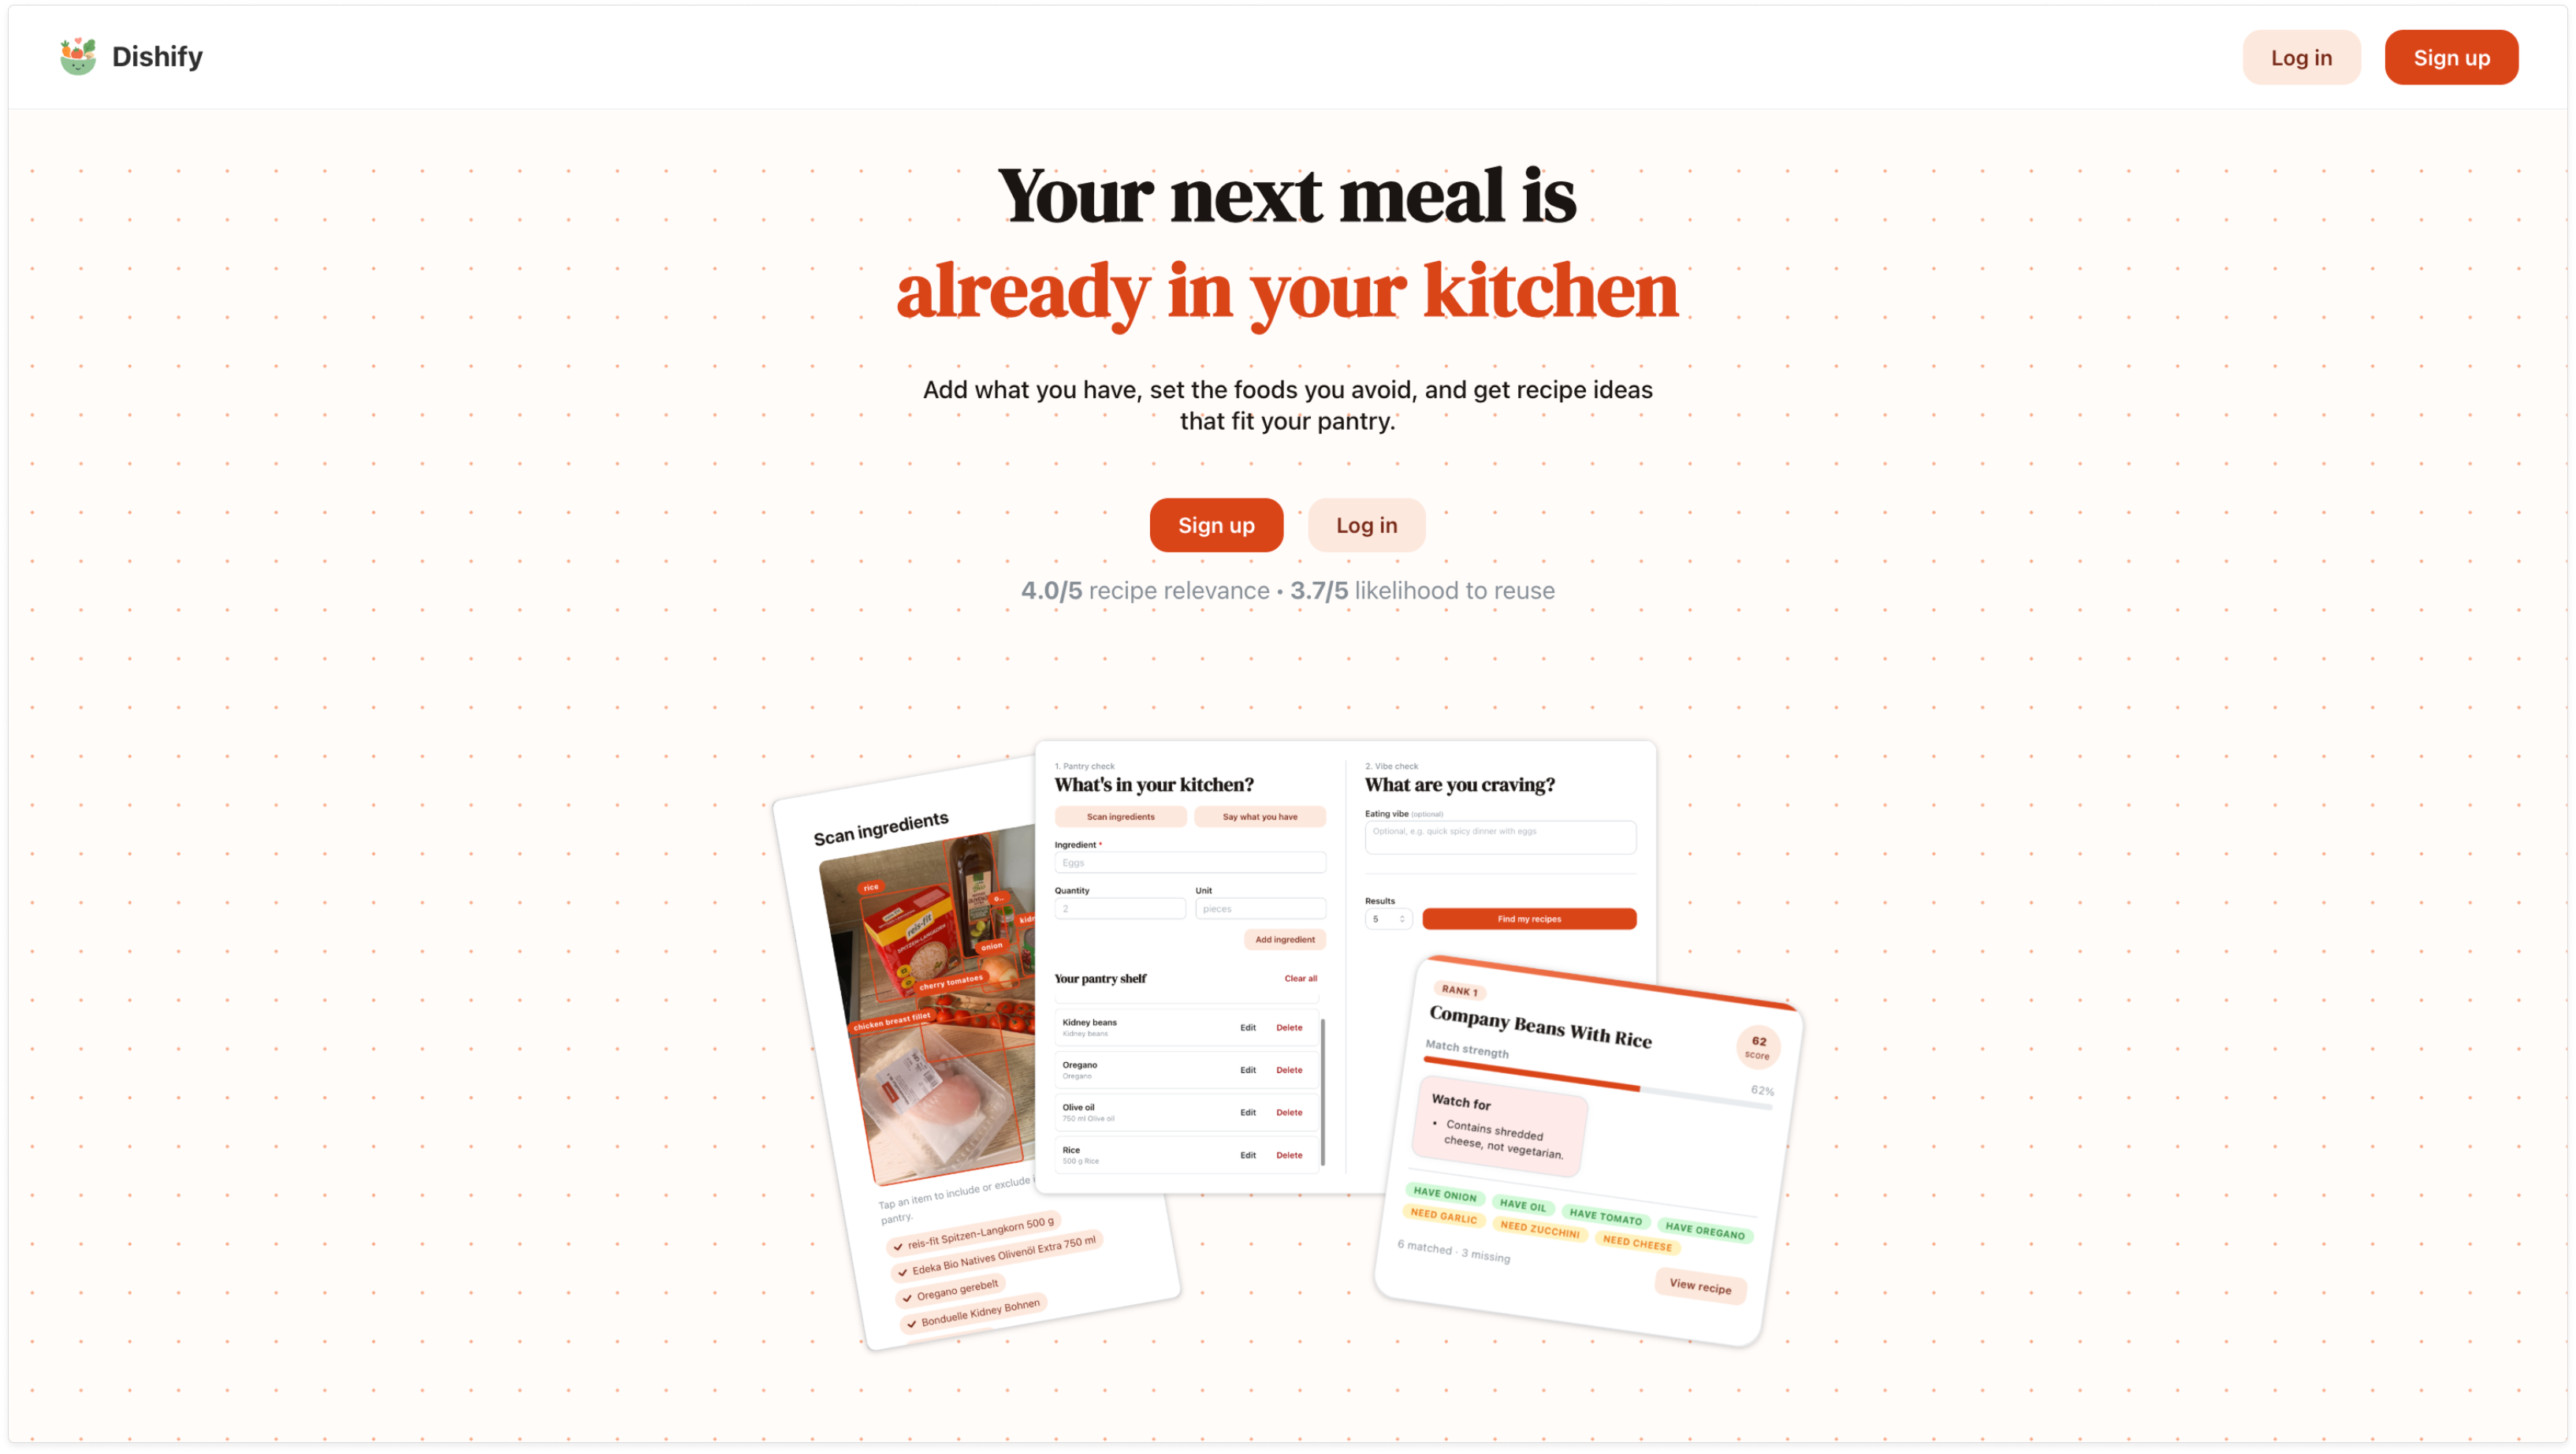
\includegraphics[width=\textwidth]{./Ressourcen/user-guide/landing-page.png}
    \captionof{figure}{The Dishify landing page.}
    \label{fig:ug-landing-page}
\end{center}

Dishify is available as an iOS app as well as on the web. Currently, only the web version is accessible. Find out more about Dishify here: \url{http://167.233.165.44}



\section{Features}

\subsection{Sign Up and Initial Preferences}
\begin{center}
    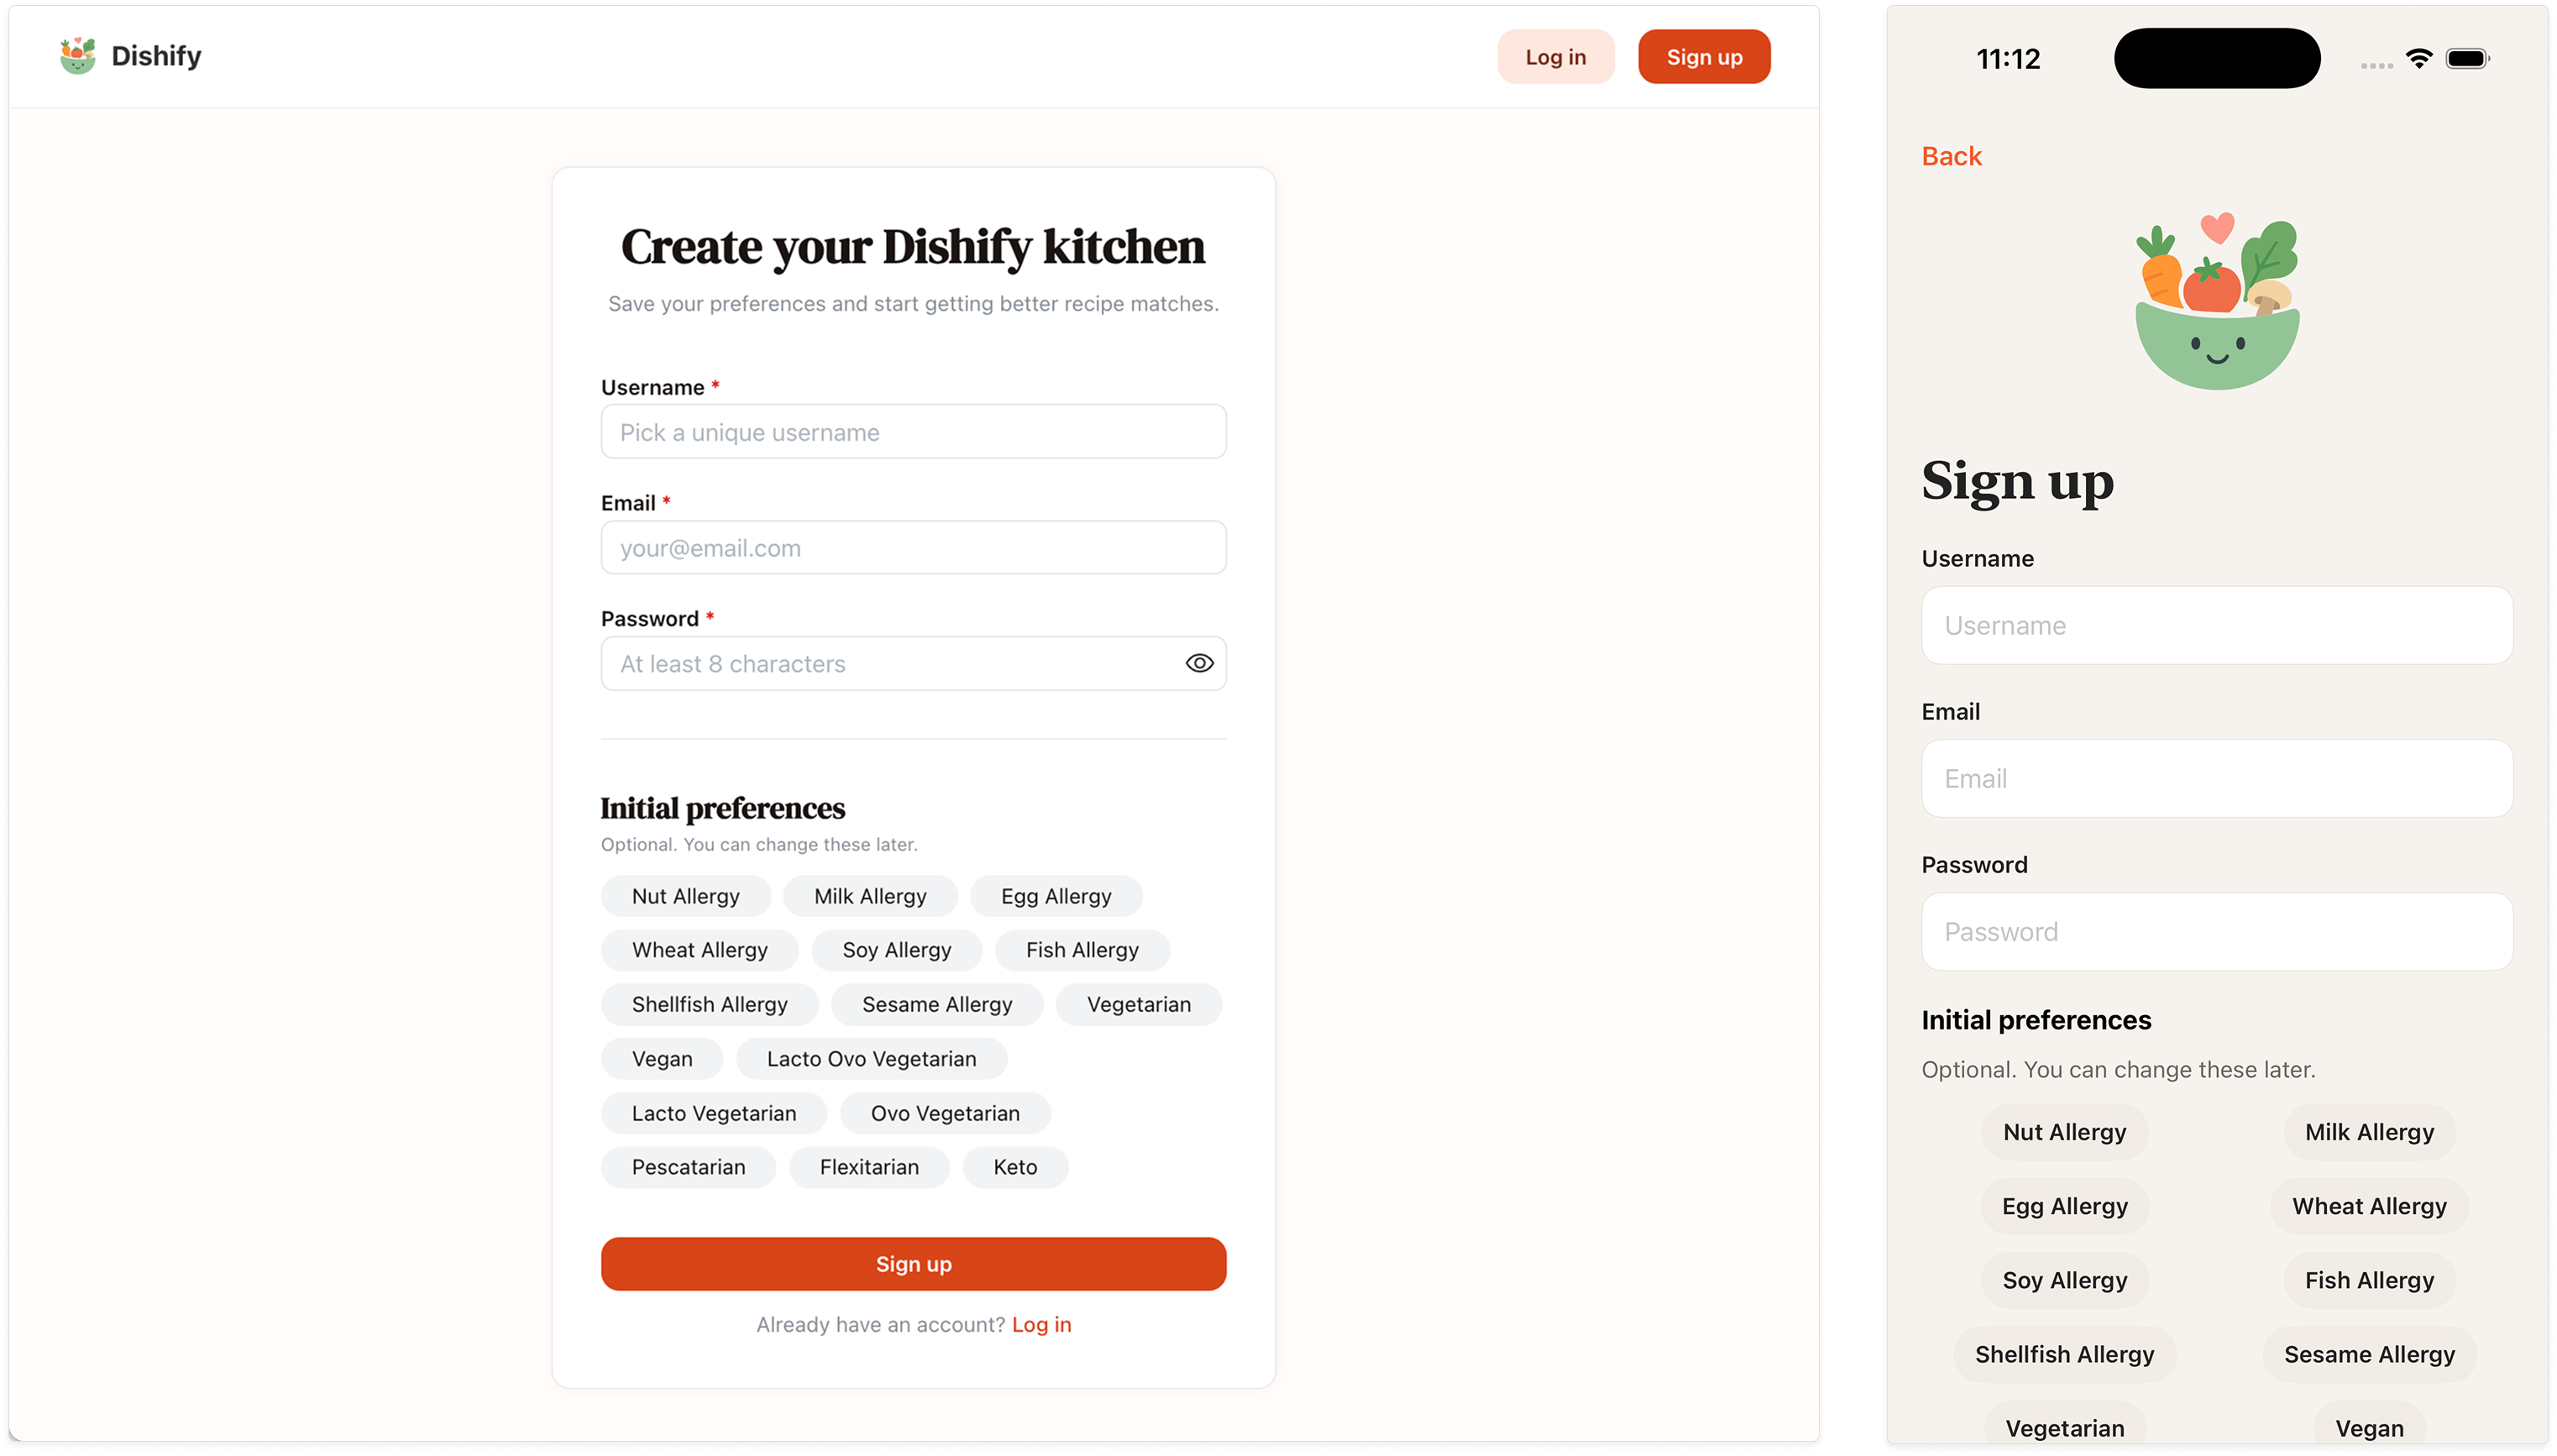
\includegraphics[width=\textwidth]{./Ressourcen/user-guide/signup-page.png}
    \captionof{figure}{The sign up page.}
    \label{fig:ug-signup}
\end{center}

During the sign up process, it is possible to specify preferences. The options include the most relevant preferences only. Additional options are available on the preferences page.



\subsection{Dietary, Allergy, and Restriction Filtering}
\begin{center}
    
\includegraphics[width=\textwidth]{./Ressourcen/user-guide/preferences.png}
    \captionof{figure}{The preferences page.}
    \label{fig:ug-preferences}
\end{center}
Dishify respects a plethora of preferences, including the categories allergies, diets, religious and ethical, medical and sensitivities, as well as ingredient exclusions.
Preferences can be changed at any time and Dishify will exclude respective recipes from its suggestions.



\subsection{Pantry-based Recipe Recommendation}
\begin{center}
    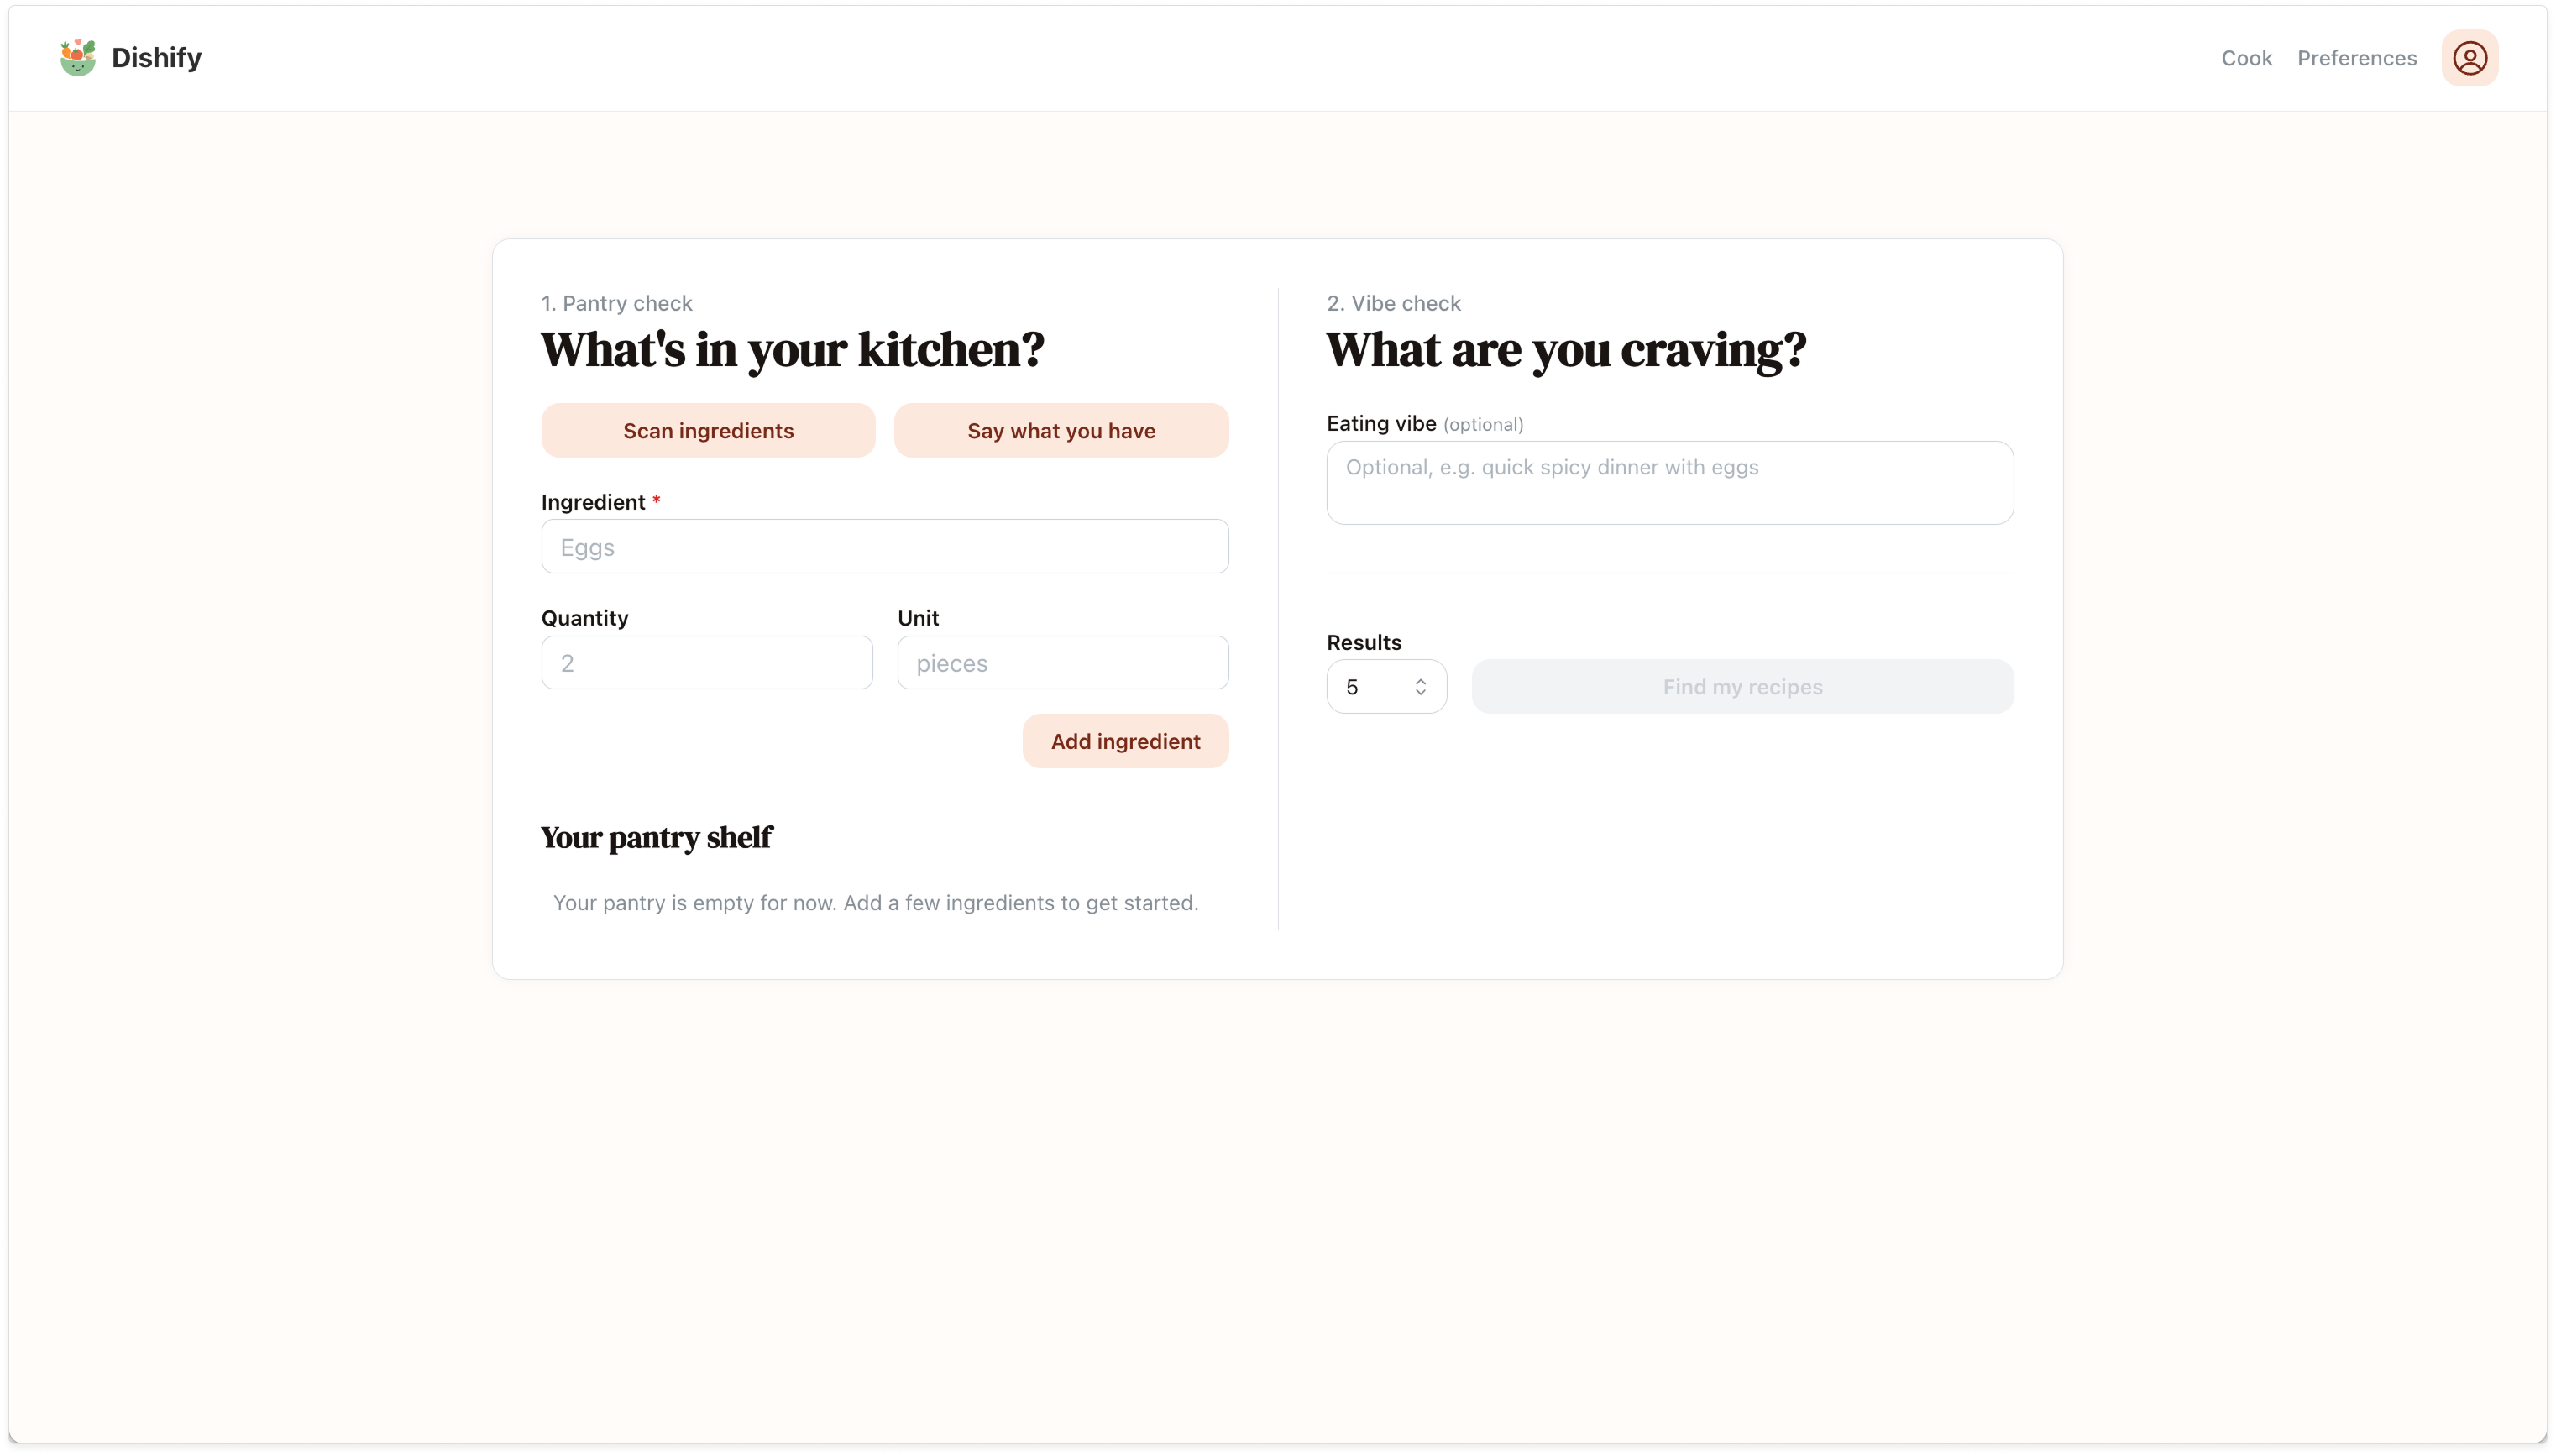
\includegraphics[width=\textwidth]{./Ressourcen/user-guide/ingredients.png}
    \captionof{figure}{The ingredients page.}
    \label{fig:ug-ingredients}
\end{center}
Dishify accepts ingredients as well as the eating vibe as input. Apart from the ingredient's name (e.g. eggs), the quantity (e.g. 2) as well as the unit of measure (e.g. pieces) can be specified.
The eating vibe (e.g. fast) provides the user with additional control over the recipe suggestions.

\begin{center}
    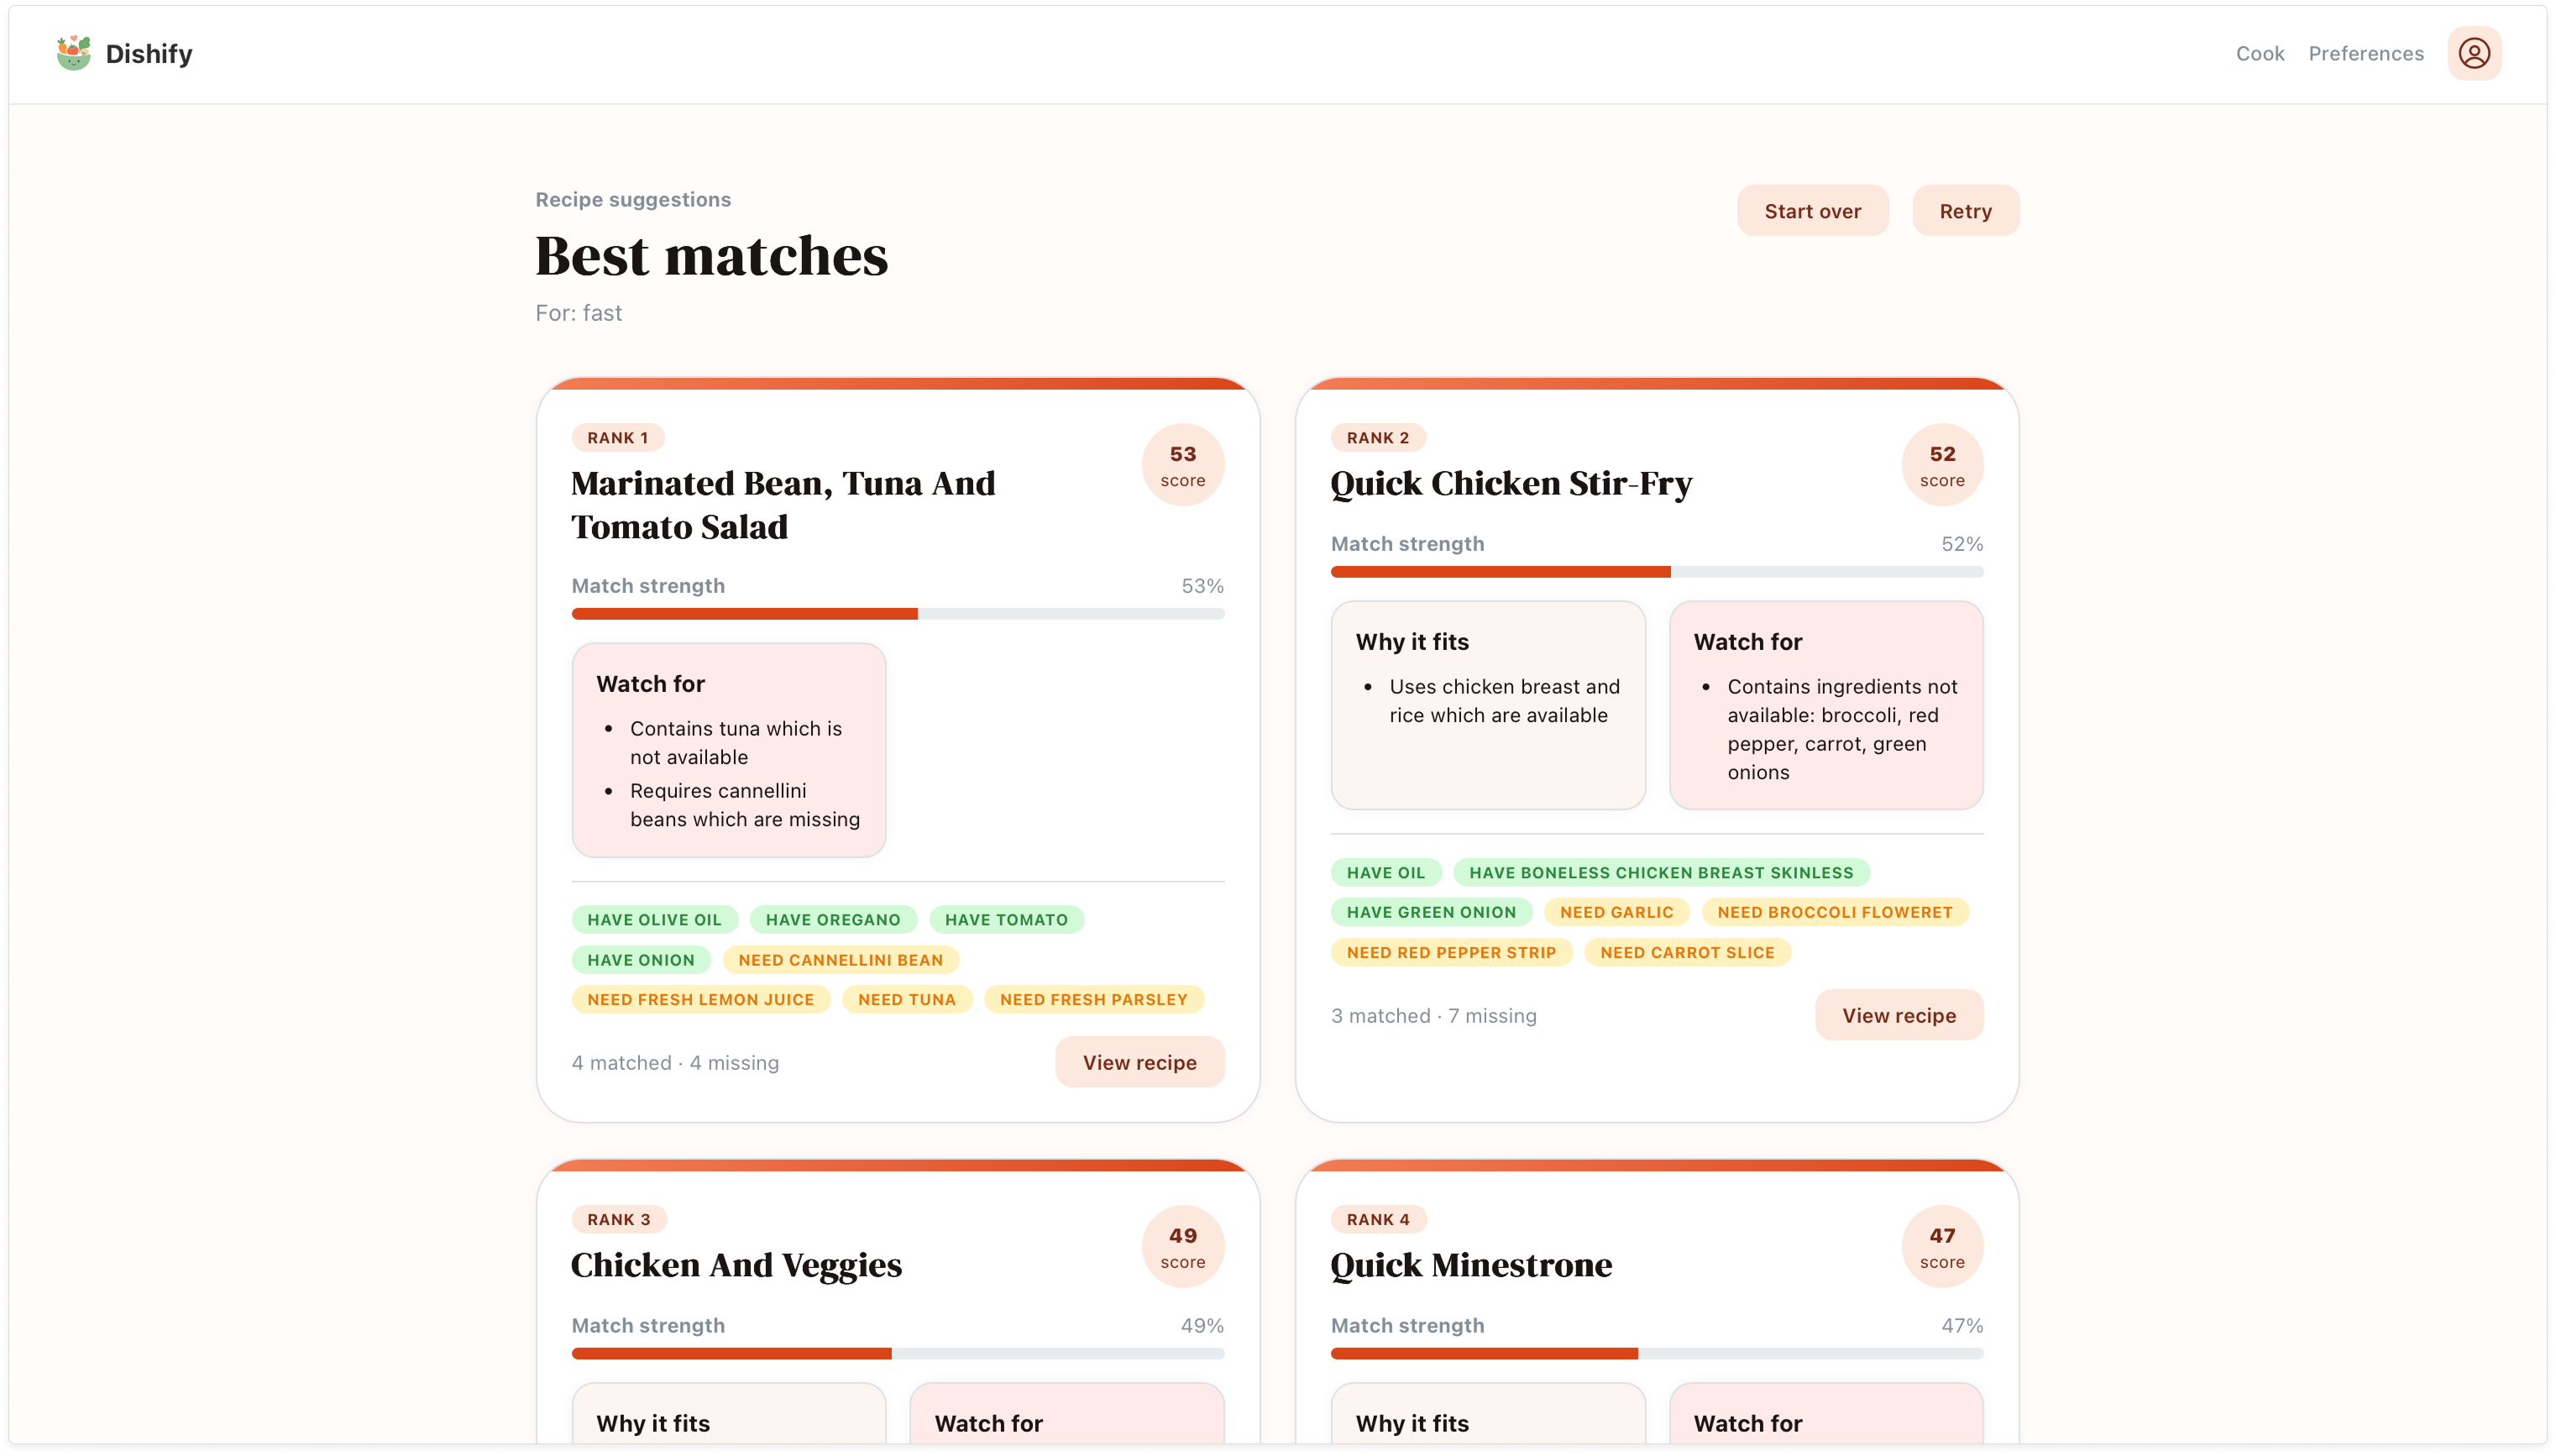
\includegraphics[width=\textwidth]{./Ressourcen/user-guide/results.png}
    \captionof{figure}{The results page.}
    \label{fig:ug-results}
\end{center}
The suggested recipes are ordered by a relevance score – a metric that shows how well a recipe fits the search and pantry: a mix of how closely it matches what you're looking for, and how many ingredients you already have on hand. 
For each suggestion Dishify displays the number of missing respectively available ingredients. Some of these ingredients are visible at a glance.



\subsection{Voice Input}
\begin{center}
    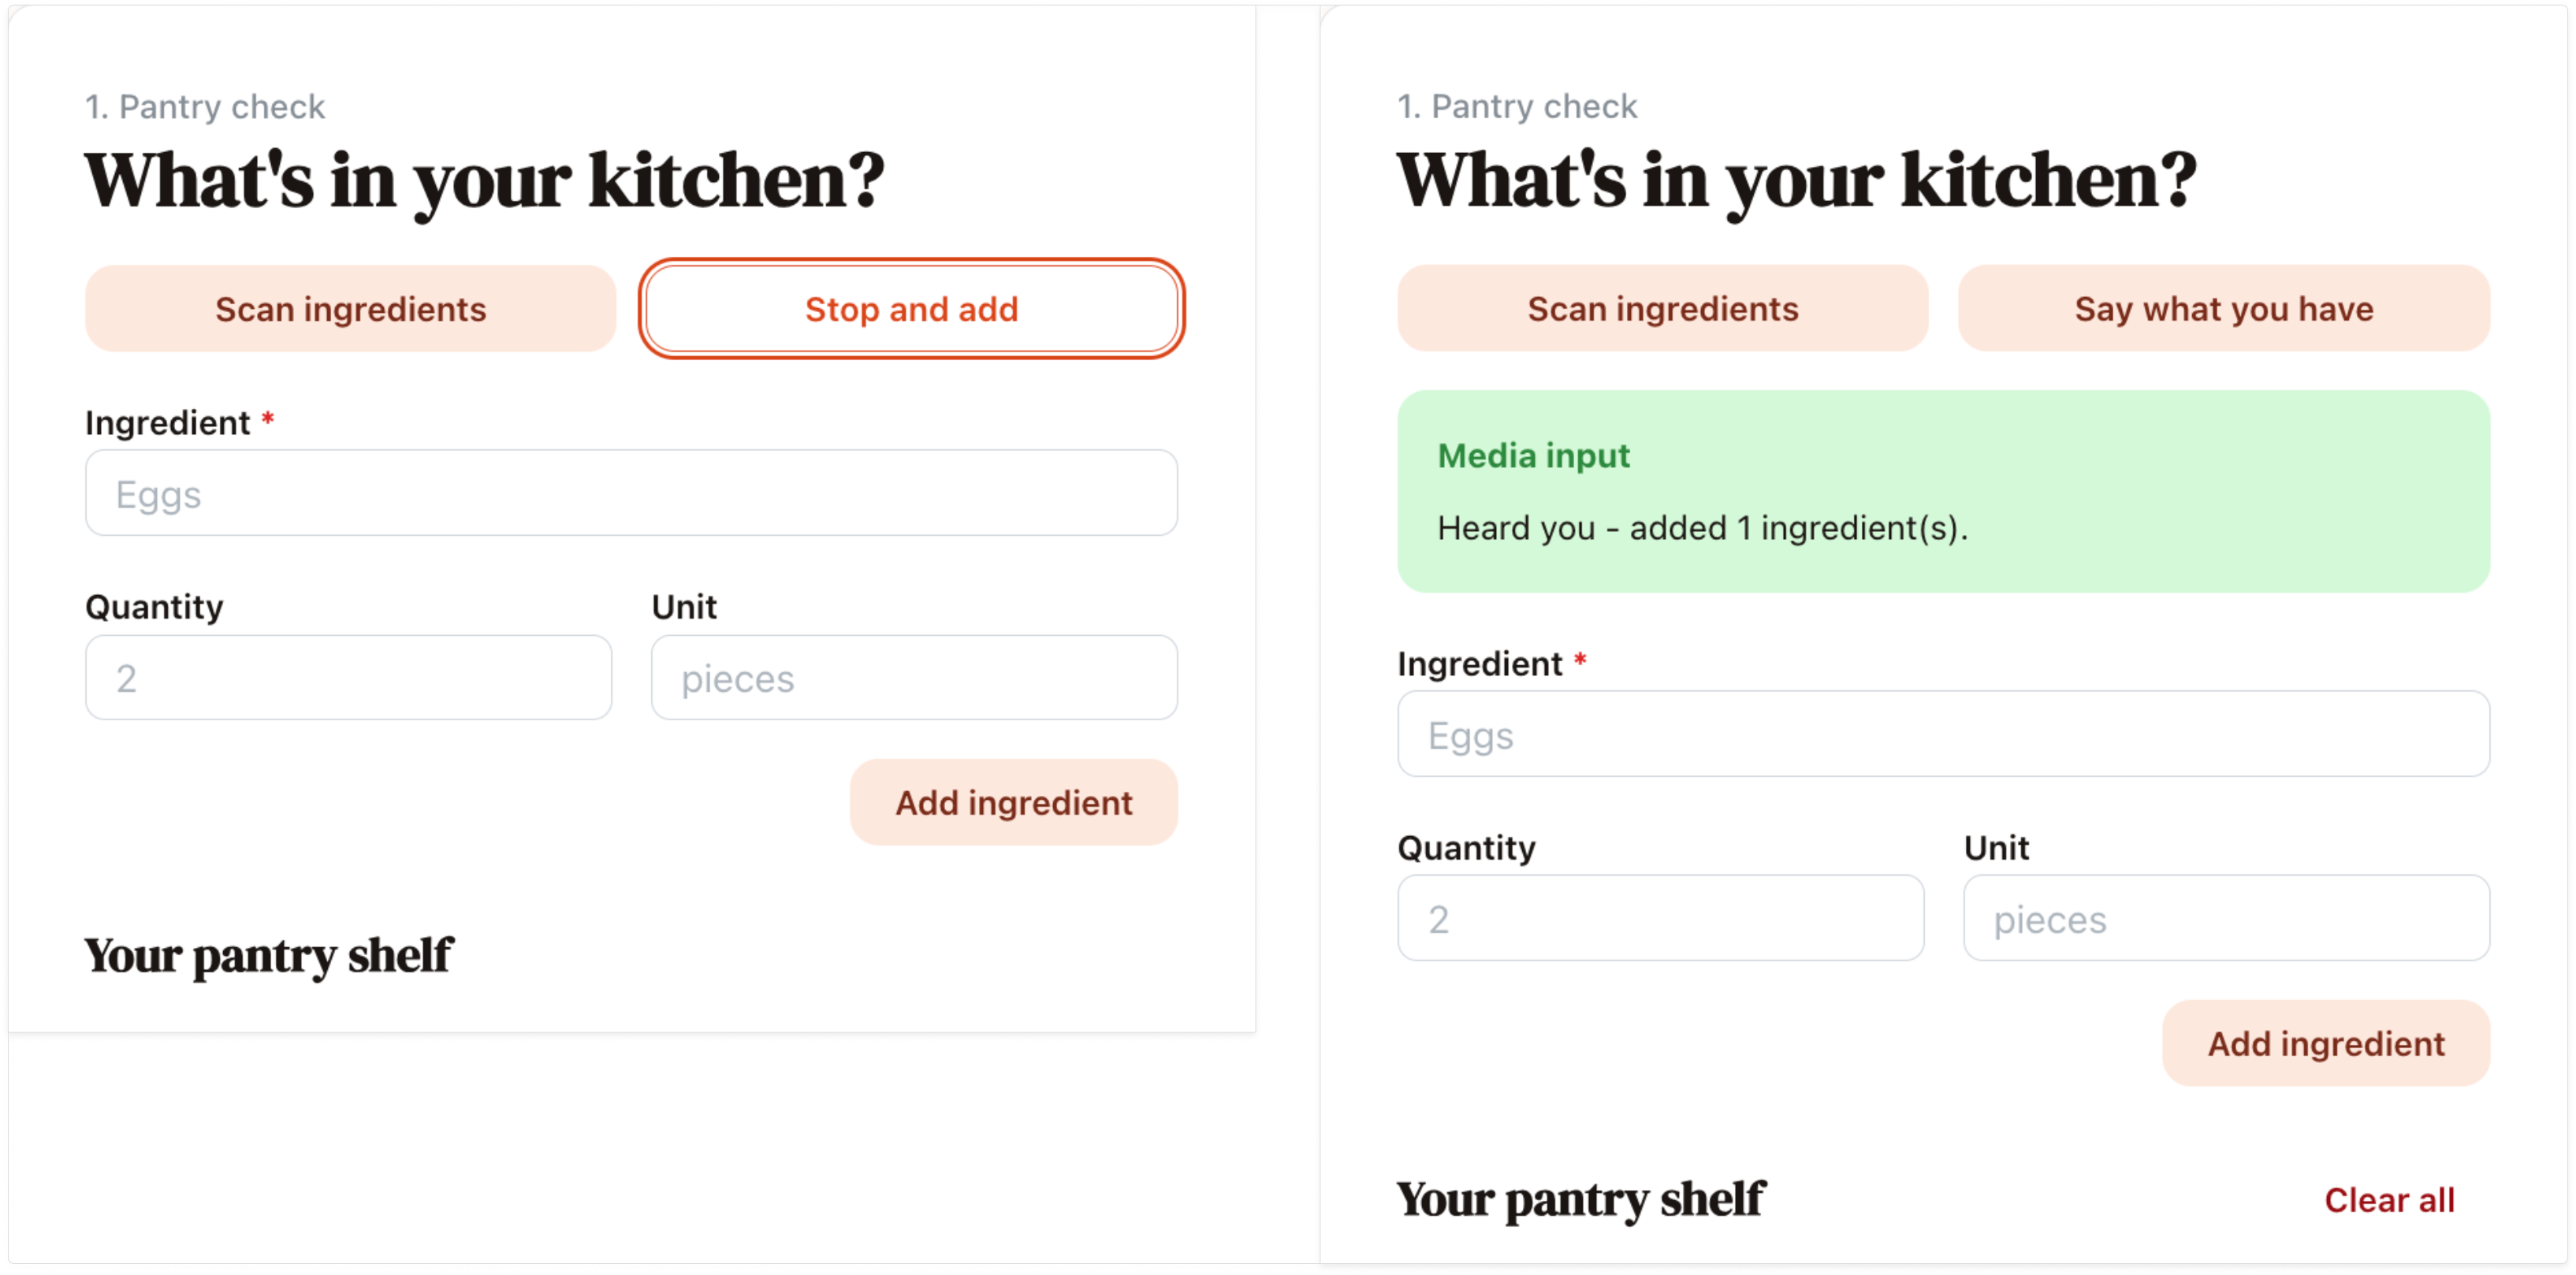
\includegraphics[width=\textwidth]{./Ressourcen/user-guide/voice.png}
    \captionof{figure}{Dishify understands voice input.}
    \label{fig:ug-voice}
\end{center}
Apart from text input Dishify understands voice input. Say what you have and Dishify adds it to the pantry shelf. 



\subsection{Image-based Ingredient Detection}
\begin{center}
    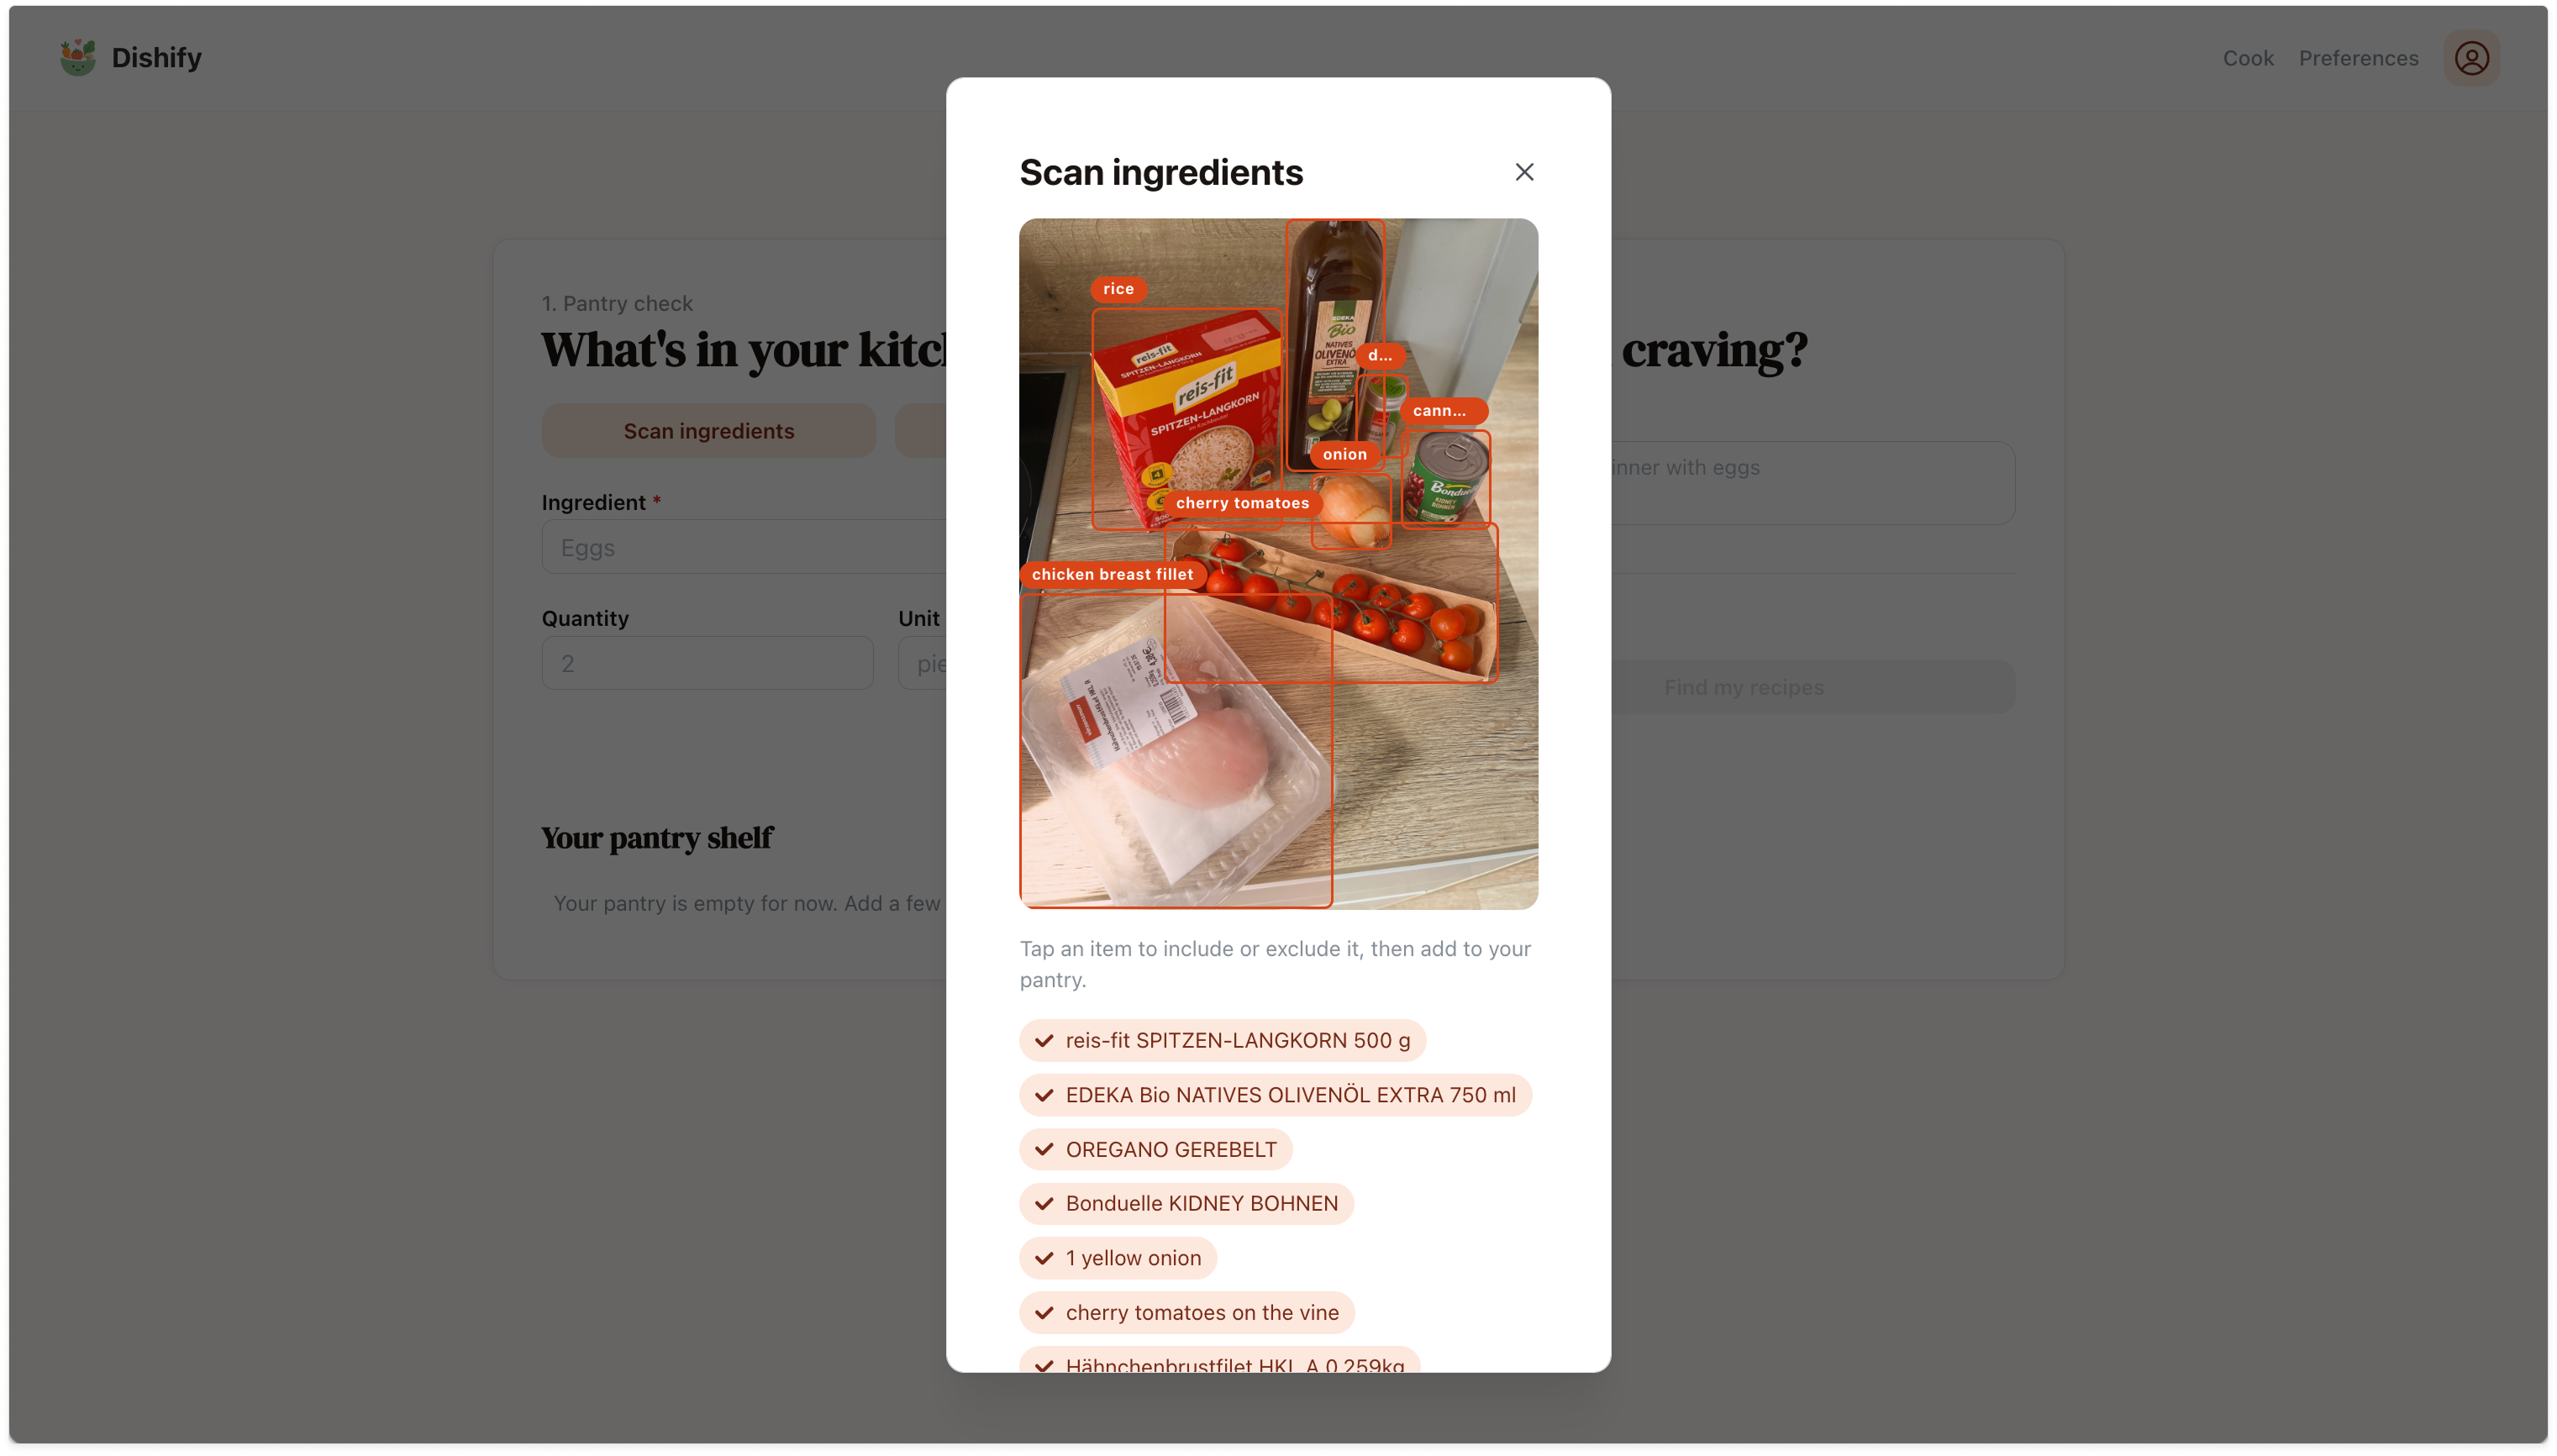
\includegraphics[width=\textwidth]{./Ressourcen/user-guide/image.png}
    \captionof{figure}{Dishify understands image input.}
    \label{fig:ug-image}
\end{center}
Dishify also allows for ingredient input via images (camera or image upload). Recognized ingredients are framed by boxes and ingredients can be deselected individually. 


\subsection{Recipe Detail}
\begin{center}
    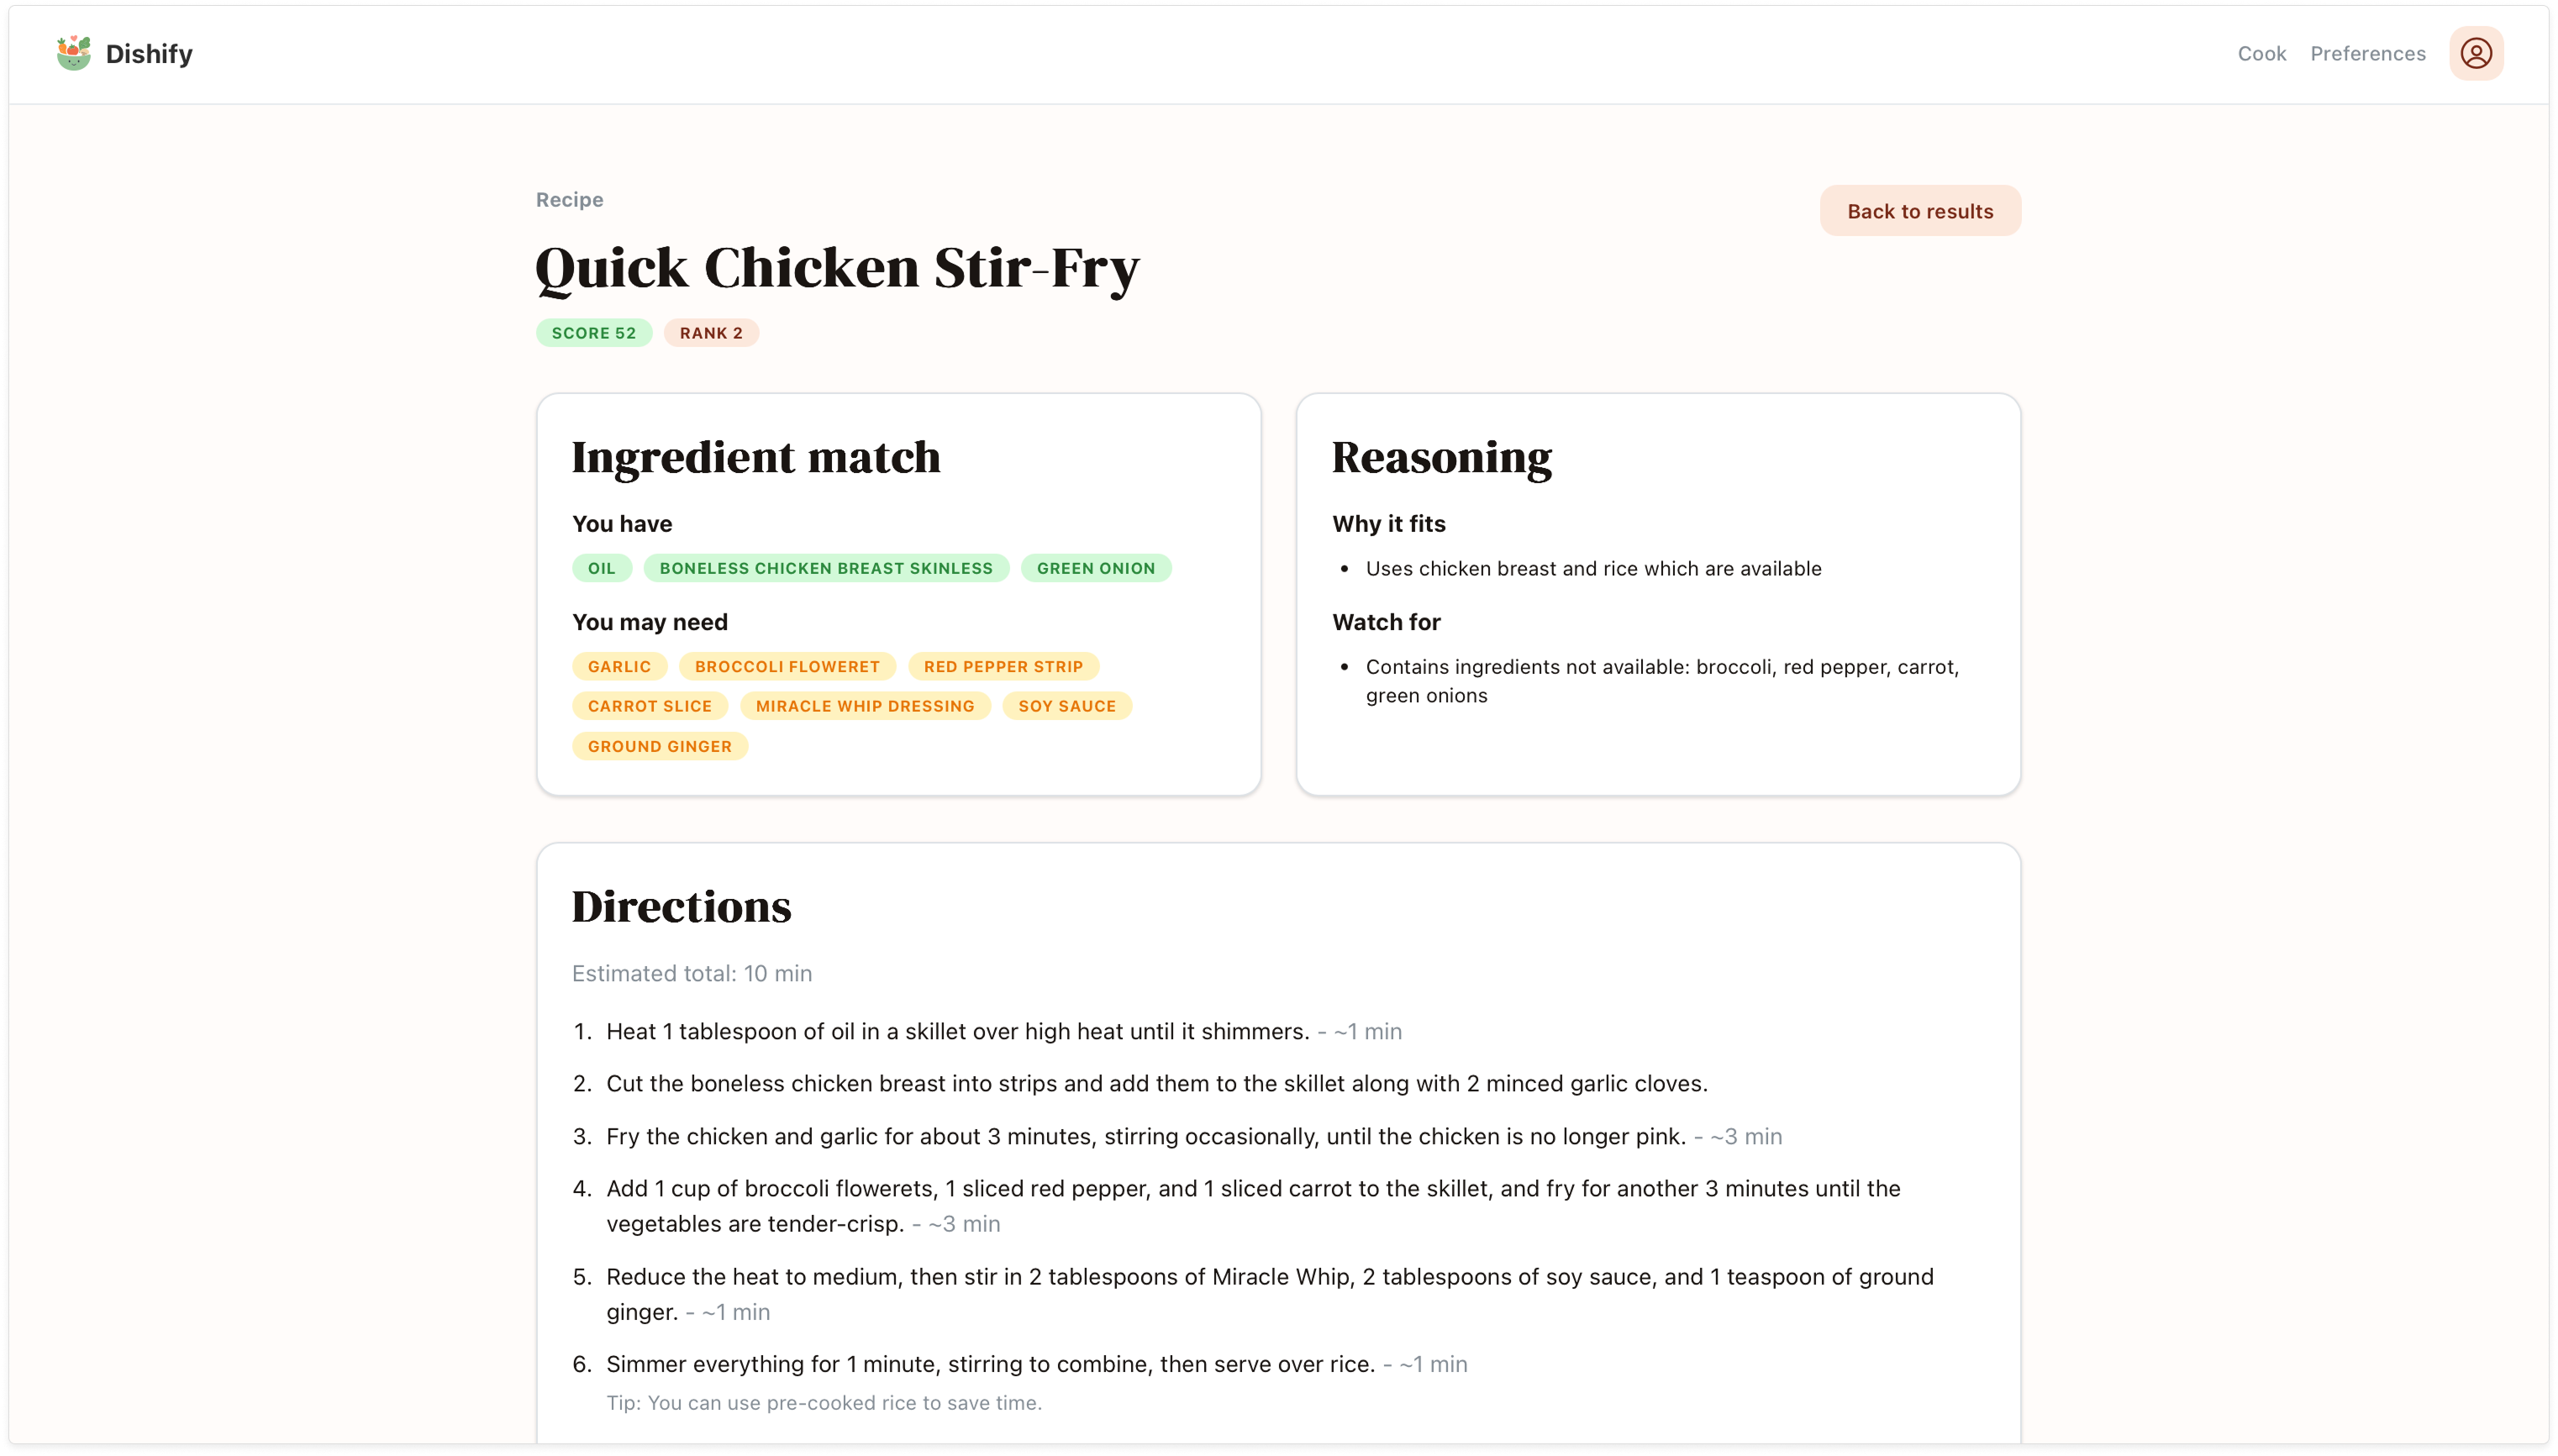
\includegraphics[width=\textwidth]{./Ressourcen/user-guide/recipe.png}
    \captionof{figure}{The recipe page.}
    \label{fig:ug-recipe}
\end{center}
The recipe page lists missing and available ingredients, an explanation why Dishify suggested the recipe, lists things to watch out for, and the steps to prepare the recipe. 
